\documentclass[a4paper,oneside,12pt]{book}

%----------------------------------------------------------------------------------------
%	README!
%   Welcome. It's worth having a read through this file
%   to set up the broad parameters, such as the name of
%   the degree, the school/department, the type of work
%   (dissertation/Final Year Project/report, etc. as well
%   as your own details.
%----------------------------------------------------------------------------------------

%----------------------------------------------------------------------------------------
%	COVER PAGE
%   The cover page is laid out in title/title.tex. You can choose a colour
%   or black and white logo
%----------------------------------------------------------------------------------------

%----------------------------------------------------------------------------------------
%	THESIS INFORMATION
%   Put title, author name, degree, type of work, school, department in here
%   It will be used for the title page and for the embedded PDF information
%----------------------------------------------------------------------------------------

\newcommand{\thesistitle}{Modern Delay-Tolerant Email} % Your thesis title, this is used in the title and abstract
\newcommand{\degree}{M.Sc. Computer Science - Future Networked Systems} % Your degree name, this is used in the title page and abstract
\newcommand{\typeofthesis}{Dissertation} % dissertation, Final Year Project, report, etc.
\newcommand{\authorname}{Rakesh Lakshmanan} % Your name, this is used in the title page and PDF stuff
%% Do not put your Student ID in the document, as TCD will not publish
%% documents that contain both your name and your Student ID.

\newcommand{\keywords}{Delay-Tolerant Networking, DTN, Email} % Keywords for your thesis
\newcommand{\school}{\href{https://www.tcd.ie/scss/}{School of Computer Science and Statistics}} % Your school's name and URL, this is used in the title page

%% Comment out the next line if you don't want a department to appear
\newcommand{\supervisor}{\href{http://www.scss.tcd.ie/}{Stephen Farrell}} % Your research group's name and URL, this is used in the title page

\AtBeginDocument{
\hypersetup{pdftitle=\thesistitle} % Set the PDF's title to your title
\hypersetup{pdfauthor=\authorname} % Set the PDF's author to your name
\hypersetup{pdfkeywords=\keywords} % Set the PDF's keywords to your keywords
\hypersetup{pdfsubject=\degree} % Set the PDF's keywords to your keywords
}

%% Language and font encodings
\usepackage[T1]{fontenc} 
\usepackage[utf8]{inputenc}
\usepackage[english]{babel}
\usepackage{lipsum}
\usepackage{ragged2e} %allows for text alignment preferences
\usepackage{float}
\usepackage{booktabs}

%% Bibliographical stuff
\usepackage[round,sort,comma,numbers]{natbib}

%% Document size
% include showframe as an option if you want to see the boxes
\usepackage[a4paper,top=2.56cm,bottom=2.56cm,left=2.56cm,right=2.56cm, head = 16pt]{geometry}
\setlength{\marginparwidth}{2cm}
%% Useful packages
\usepackage{amsmath}
\usepackage[autostyle=true]{csquotes} % Required to generate language-dependent quotes in the bibliography
\usepackage[pdftex]{graphicx}
\usepackage[colorinlistoftodos]{todonotes}
\usepackage[colorlinks=true, allcolors=black]{hyperref}
\usepackage{float}
\makeatletter\renewcommand{\fps@table}{tbp}\makeatletter

% 插入 Bash 代码
\usepackage{listings}
\usepackage{xcolor}
\lstdefinelanguage{bash}{
  morekeywords={docker, echo, cat},
  sensitive=true,
  morecomment=[l]{\#},
  morestring=[b]",
}

\lstset{
  language=bash,
  basicstyle=\ttfamily\small,
  keywordstyle=\color{blue},
  commentstyle=\color{gray},
  stringstyle=\color{orange},
  showstringspaces=false,
  columns=fullflexible,
  breaklines=true,
  frame=single,
  captionpos=b
}
\usepackage{array}

\usepackage{caption} % if no caption, no colon
%\usepackage{sfmath} %use sans-serif in the maths sections too
\usepackage[parfill]{parskip}    % Begin paragraphs with an empty line rather than an indent
\usepackage{setspace} % to permit one-and-a-half or double spacing
\usepackage{enumerate} % fancy enumerations like (i) (ii) or (a) (b) and suchlike
\usepackage{booktabs} % To thicken table lines
\usepackage{fancyhdr}

%\pagestyle{plain} % Embrace simplicity!

%% The Mechanical engineers require your name and ID on the top of every page.
%% Uncomment the following block if you want your name and ID at the top of
%% (almost) every page.

\pagestyle{fancy}
\fancyhf{} % sets both header and footer to nothing
\renewcommand{\headrulewidth}{0pt}
\cfoot{\thepage}
%\ifdefined\authorid
%\chead{\it \authorname\ (\authorid)}
%\else
%\chead{\it \authorname}
%\fi
%% End of block

%% It is not a requirement of the university that the font should be sans-serif, but
%% the Mechanical engineers require it. Comment out the following line to disable it
%%\renewcommand{\familydefault}{\sfdefault} %use the sans-serif font as default

%% If you're not using sans-serif, consider using Palatino instead of the LaTeX standard
\usepackage{mathpazo} % Use the Palatino font by default if you prefer it to Computer Modern

\renewcommand{\theequation}{\arabic{equation}} %% use continuous equation numbers

%% Format Chapter headings appropriately
\usepackage{titlesec}
\definecolor{tcdblue}{cmyk}{0.94, 0.38, 0, 0.27}
\newcommand{\hsp}{\hspace{20pt}}
\titleformat{\chapter}[hang]{\Huge\bfseries}{\thechapter\hsp\textcolor{tcdblue}{|}\hsp}{0pt}{\Huge\bfseries}

\title{\thesistitle}
\author{\authorname}

\frontmatter
\begin{document}
\input{title/title.tex}
\pagenumbering{roman}
\doublespacing

% \section*{Declaration}
% I hereby declare that this \typeofthesis\ is entirely my own work and that it has not been submitted as an exercise for a degree at this or any other university.

% I have read and I understand the plagiarism provisions in the General Regulations of the University Calendar for the current year, found at \url{http://www.tcd.ie/calendar}.

% I have also completed the Online Tutorial on avoiding plagiarism `Ready Steady Write', located at \url{http://tcd-ie.libguides.com/plagiarism/ready-steady-write}.
% \vspace{1cm}

% Signed:~\rule{5cm}{0.3pt}\hfill Date:~\rule{5cm}{0.3pt}


\newpage
\chapter{Abstract}
% A short summary of the problem investigated, the approach taken and the key findings. This should not be more that around 400 words.

% The must be on a separate page.

% what’s the title for our title
% abstract one page
% five paragraphs 
% area and digital twin
% project research questions
% two paragraphs how to solve them 
% paragraph to implement and evaluate
% main findings one paragraphs
% expanding the abstract


% introduction
% literature review 
% design implementation
% evaluation
% conclusion

Deep-space links carry long delays and go down for long stretches, so the protocols that assume a fast, always-on connection do not work across them. Delay-Tolerant Networking (DTN) makes it possible to move email over such links, but the spam filtering that any real mail service needs has never been studied under these conditions. This matters because every filter leans on live lookups to remote servers, and those lookups now have to cross the delayed link.

This work measures how three widely used anti-spam tools: SpamAssassin, rspamd, and Vipul's Razor, behave when their traffic runs over a DTN link, and explains why. A three-node Earth–Moon testbed was built from real software: Postfix and Dovecot for mail, ION-DTN and the BPMail gateway for transport, and a private DNS resolver for the blocklist queries. A one-way delay of 1.3 seconds was applied on the relay, and each tool was run over a corpus of 681 messages, once with delay and once without, while recording per-message verdicts, scan times, and packet captures.

The tools do not cope with delay on their own. A blocklist answer that arrives one round-trip late is thrown away by the resolver unless its timers are raised above the delay, and when that is not done the filter still runs, still scores the message, and quietly lets spam through. Cutting a tool's own timeout below the round-trip does not trade a little detection for speed; it removes detection outright, and a tool that relies on a single remote service stops returning any verdict. In every case the filter's own lookups put far more traffic on the link than the mail they inspect. These results hold at Moon distance and grow worse toward Mars, where the round-trip exceeds every timeout in the stack, so filtering of this kind cannot be carried to interplanetary links without moving the checks off the live path.


\newpage
\raggedright %\raggedright turns off justification and hypenation

\section*{\Huge{Acknowledgements}}
I would like to thank my supervisor, Professor Stephen Farrell. Under his supervision, I was able to successfully complete this dissertation. His inspiration and suggestions regarding the project's direction were essential for the progress of this research.

I am also grateful to my family and friends for their support and encouragement throughout this process.
\newpage \listoffigures
\newpage \listoftables
\newpage
\chapter*{List of Abbreviations}
\begin{singlespace}
\begin{tabular}{ll}
\toprule
\textbf{Abbreviation} & \textbf{Expansion} \\
\midrule
ARM64  & 64-bit ARM Architecture \\
BP     & Bundle Protocol \\
DKIM   & DomainKeys Identified Mail \\
DMARC  & Domain-based Message Authentication, Reporting, and Conformance \\
DNS    & Domain Name System \\
DNSBL  & DNS-based Blocklist \\
DNSSEC & Domain Name System Security Extensions \\
DTN    & Delay-Tolerant Networking \\
DTPC   & Delay-Tolerant Payload Conditioning \\
HTTP   & Hypertext Transfer Protocol \\
IETF   & Internet Engineering Task Force \\
ifb    & Intermediate Functional Block \\
IMAP   & Internet Message Access Protocol \\
ION    & Interplanetary Overlay Network \\
LTS    & Long-Term Support \\
NAT    & Network Address Translation \\
RTO    & Retransmission Timeout \\
RTT    & Round-Trip Time \\
SDR    & Simple Data Recorder (ION persistent store) \\
SMTP   & Simple Mail Transfer Protocol \\
SPF    & Sender Policy Framework \\
SSH    & Secure Shell \\
SYN    & Synchronize (TCP segment) \\
TCP    & Transmission Control Protocol \\
TLS    & Transport Layer Security \\
UDP    & User Datagram Protocol \\
URI    & Uniform Resource Identifier \\
URIBL  & URI-based Blocklist \\
VM     & Virtual Machine \\
\bottomrule
\end{tabular}
\end{singlespace}
% \newpage
% \section*{\Huge{Nomenclature}}
% \begin{tabular}{lp{9cm}l}
% A&Area of the wing&$m^{2}$\\
% B\\
% C& Roman letters first, with capitals\ldots\\
% a&then lower case.\\
% b\\
% c\\
% $\Gamma$&Followed by Greek capitals\ldots\\
% $\alpha$&then lower case greek symbols.\\
% $\beta$\\
% $\epsilon$\\
% TLA&Finally, three letter acronyms and other abbreviations arranged alphabetically\\
% \end{tabular}
% \vspace{2cm}

% If a parameter has a typical unit that is used throughout your report, then it should be included here on the right hand side.

% If you have a very mathematical report, then you may wish to divide the nomenclature list into functions and variables, and then sub- and super-scripts.

% Note that Roman mathematical symbols are typically in a serif font in italics.

\mainmatter
\input{introduction/introduction.tex}
\input{Report/Literature Review/Literature Review}
\chapter{System Design}


This chapter describes the testbed used to evaluate anti-spam tools under one-way delay representing a deep-space DTN link. It sets out the node layout, the host model and the reasons for it, the tools under test, the DTN configuration, the delay simulation, and the experimental design.

\section{System Architecture}
\label{sec:arch}

The testbed has two networks joined by a relay. Each node runs an ION instance (Section~\ref{sec:background-ion}) and is a separate virtual machine running Ubuntu 22.04 LTS. Earth uses 192.168.100.0/24 and Moon uses 192.168.200.0/24. The nodes are:

\begin{itemize}
  \item \textbf{Mail1 (Earth).} The Earth mail server. Runs Postfix and Dovecot. Address 192.168.100.10.
  ION node 1.
  \item \textbf{Space (Relay).} The transit node between the two networks. Runs an
  ION node and carries the delay and packet-capture configuration. Earth-side
  interface 192.168.100.1, Moon-side interface 192.168.200.1. ION node 2.
  \item \textbf{Mail2 (Moon).} The Moon mail server. Runs Postfix, Dovecot, and
  the three anti-spam tools. Address 192.168.200.11. ION node 3.
  \item \textbf{Client1 (Earth).} User terminal on the Earth network. Runs Thunderbird and a script (the test harness)(Section~\ref{sec:harness}) that injects the spam messages. Connects to Mail1 over IMAP (port 143) and SMTP submission (port 587, STARTTLS).
  \item \textbf{Client2 (Moon).} User terminal on the Moon network. Runs
  Thunderbird and connects to Mail2 the same way.
\end{itemize}

Mail moves server to server across the DTN link: a message submitted on one mail server is carried as a bundle through the relay to the other. ION runs on all three servers, so the bundle path is node 1 (Earth) to node 2 (relay) to node 3 (Moon). The relay is the only path between the two networks, so all traffic between Earth and Moon passes through it. This is where the one-way link delay is applied, standing in for the Earth–Moon propagation time. Mailboxes use mbox format, and each user reads mail from their local server. The topology is shown in Figure~\ref{fig:topology}.

\begin{figure}[ht]
\centering
\resizebox{\textwidth}{!}{%
\begin{tikzpicture}[
  font=\small,
  box/.style={draw, rounded corners, align=center, minimum width=3.2cm, minimum height=1.5cm},
  cl/.style={draw, rounded corners, align=center, minimum width=3.2cm, minimum height=1cm},
  >={Stealth[]}
]
\node[box] (mail1) {\textbf{Mail1 -- Earth}\\Mail Server: Postfix, Dovecot\\IP: 192.168.100.10\\ION node: 1};
\node[cl, below=1.2cm of mail1] (client1) {\textbf{Client1 -- Earth}\\Thunderbird};
\node[box, right=2.6cm of mail1] (relay) {\textbf{Space -- Relay}\\Delay + capture\\IP: 192.168.100.1 / 192.168.200.1\\ION node: 2};

\node[box, right=2.6cm of relay] (mail2) {\textbf{Mail2 -- Moon}\\Mail Server: Postfix, Dovecot\\IP: 192.168.200.11\\ION node: 3};
\node[cl, below=1.2cm of mail2] (client2) {\textbf{Client2 -- Moon}\\Thunderbird};
\draw[<->, thick] (client1) -- node[right, font=\footnotesize]{IMAP / SMTP} (mail1);
\draw[<->, thick] (mail1) -- (relay);
\draw[<->, thick] (relay) -- node[above, font=\footnotesize, align=center]{DTN link\\(delay)} (mail2);
\draw[<->, thick] (client2) -- node[right, font=\footnotesize]{IMAP / SMTP} (mail2);
\end{tikzpicture}%
}
\caption{Testbed topology. Each client connects only to its local mail server. The
relay is the only path between the Earth and Moon networks and is where the one-way
link delay is applied.}
\label{fig:topology}
\end{figure}


\paragraph{Data flow (Earth to Moon).}
The path of a message is shown in Figure~\ref{fig:dataflow}.

\begin{figure}[H]
\centering
\begin{tikzpicture}[
  font=\small, >={Stealth[]},
  flowstep/.style={draw, rounded corners, align=center, minimum width=8.5cm, minimum height=0.85cm},
  node distance=0.45cm
]
\node[flowstep] (s1) {User writes the message in Thunderbird on Client1 (Earth)};
\node[flowstep, below=of s1] (s2) {Client1 submits it to Postfix on Mail1 over SMTP};
\node[flowstep, below=of s2] (s3) {Mail1 hands the message to its ION node (node 1)};
\node[flowstep, below=of s3] (s4) {ION encapsulates the message into a bundle};
\node[flowstep, dashed, below=of s4] (s5) {Bundle is forwarded through Space (node 2) : one-way delay applied};
\node[flowstep, below=of s5] (s6) {ION on Mail2 (node 3) receives the bundle and rebuilds the message (Moon)};
\node[flowstep, below=of s6] (s7) {Postfix and Dovecot on Mail2 deliver it to the recipient's mailbox.};
\node[flowstep, below=of s7] (s8) {User reads it in Thunderbird on Client2 over IMAP};
\foreach \a/\b in {s1/s2,s2/s3,s3/s4,s4/s5,s5/s6,s6/s7,s7/s8} \draw[->] (\a) -- (\b);
\end{tikzpicture}
\caption{End-to-end path of an email from Earth to Moon across the DTN link.}
\label{fig:dataflow}
\end{figure}

\section{Environment and Technology Selection}
\label{sec:env}

\subsection{Virtual machines over containers}
The testbed runs on full virtual machines (Ubuntu 22.04 LTS, ARM64, under UTM on macOS). Containers were considered but not used. They were not used for three reasons:

\begin{itemize}
   \item \textbf{VMs match the topology.} The testbed mimics three separate machines — Earth, Space, Moon — connected by a long-delay link, and full VMs naturally model this, whereas containers share one kernel on one host.
  \item \textbf{Simpler delay setup.} Setting up an intermediate functional block (ifb), the virtual device used to apply delay to incoming traffic (Section~\ref{sec:delay}), is fiddly and error-prone inside containers, but it is straightforward on a VM where each node has its own kernel and network stack.
  \item \textbf{DTN state stays isolated per node.} Each ION node keeps its own bundle store and contact schedule, and a full VM ensures the link delay sits on the path itself rather than leaking into a node's own processing.
\end{itemize}

\section{Email stack}
\begin{itemize}
  \item \textbf{Postfix} was chosen for its clear interface for handing mail to an external program, needed to pass messages to the DTN layer.
  \item \textbf{Dovecot} was chosen because it works directly with mbox format and the local system accounts that Postfix delivers to.
  \item \textbf{Thunderbird}was chosen as a standard mail client, so the message traffic in the testbed matches what a normal user would generate.
\end{itemize}

\section{DTN stack}
\begin{itemize}
  \item \textbf{ION-DTN}was chosen for its deep-space flight heritage and its existing tool for carrying email over the Bundle Protocol, which connects directly to the mail stack.
\end{itemize}

\section{Anti-Spam Tool Selection}
\label{sec:tools}

Three tools were selected, each with a different external dependency:

\begin{itemize}
  \item \textbf{SpamAssassin 3.4.6} --- content scoring that depends on DNS
  blocklist lookups.
  \item \textbf{rspamd 2.7} --- content scoring with a large number of
  asynchronous DNS lookups.
  \item \textbf{Vipul's Razor 2.84} --- collaborative filtering that checks each message against a central catalogue server, which holds signatures of known spam reported by other users.
\end{itemize}

The three cover the main ways a filter reaches the network: blocklist DNS (SpamAssassin, rspamd) and a TCP request to a central reputation server (Razor). Testing one tool would show only one failure path.


\section{DTN Design}
\label{sec:dtn}
The DTN layer uses ION-DTN 4.1.4~\cite{ionsoftware} and BPMail. The three servers run ION as nodes on a single ipn scheme (Section~\ref{sec:background-dtn}): Mail1 (Earth) is node 1, Space (relay) is node 2, and Mail2 (Moon) is node 3. Bundles are carried over a UDP convergence layer (Section~\ref{sec:background-dtn}), with each node listening on its own port: 1113 on Mail1, 2113 on Space, and 3113 on Mail2. The relay forwards bundles between the two mail nodes, so the path from Earth to Moon is node 1 to node 2 to node 3. The contact plan (Section~\ref{sec:background-ion}) sets the windows during which the nodes can exchange bundles. BPMail sits above ION on each mail server: it takes a message from Postfix, encapsulates it into a bundle for the destination node, and rebuilds it on arrival. The full configuration, including the SDR settings (Section~\ref{sec:background-ion}), the contact plan, and the startup order, is given in the implementation chapter.

\section{Delay Simulation Design}
\label{sec:delay}
Delay is applied with netem on the relay, to all traffic crossing the boundary between the Earth and Moon networks. An Earth–Moon link delays travel in both directions: a signal takes about 1.3 seconds each way, so a round-trip takes about 2.6 seconds. The testbed emulates this by delaying each leg on the relay's Moon-facing interface.

The complication is that \texttt{tc} can only shape traffic \emph{leaving} an interface, so the two legs have to be handled separately. The Earth-to-Moon leg is the egress direction on that interface and is delayed by a netem qdisc attached to the interface root. The Moon-to-Earth leg arrives as ingress, and ingress has no egress queue to attach a qdisc to. To delay it, incoming traffic is redirected to an Intermediate Functional Block (ifb) device, whose own egress path can be shaped normally, and the same netem delay is applied there. The two mechanisms, the root qdisc and the ifb device are therefore the two halves of a single symmetric delay, not a way to delay one direction while sparing the other. Traffic that stays within a single network never reaches the relay and is unaffected. This is shown in Figure~\ref{fig:ifb}.



\begin{figure}[ht]
\centering
\resizebox{0.95\textwidth}{!}{%
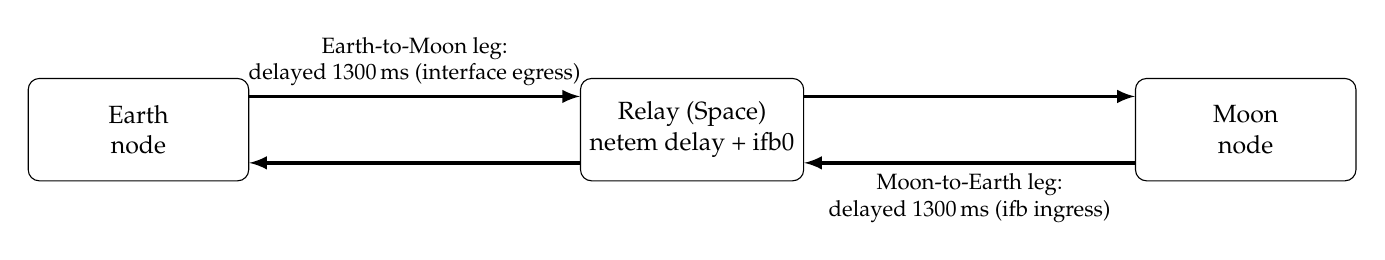
\begin{tikzpicture}[
  font=\small,
  box/.style={draw, rounded corners, align=center, minimum width=2.8cm, minimum height=1.3cm}
]
\node[box] (earth) {Earth\\node};
\node[box, right=4.2cm of earth] (relay) {Relay (Space)\\netem delay + ifb0};
\node[box, right=4.2cm of relay] (moon) {Moon\\node};

% Earth-to-Moon leg (top row, left to right)
\draw[-latex, very thick] ([yshift=12pt]earth.east) -- node[above, font=\footnotesize, align=center]{Earth-to-Moon leg:\\delayed 1300\,ms (interface egress)} ([yshift=12pt]relay.west);
\draw[-latex, very thick] ([yshift=12pt]relay.east) -- ([yshift=12pt]moon.west);

% Moon-to-Earth leg (bottom row, right to left)
\draw[-latex, very thick] ([yshift=-12pt]moon.west) -- node[below, font=\footnotesize, align=center]{Moon-to-Earth leg:\\delayed 1300\,ms (ifb ingress)} ([yshift=-12pt]relay.east);
\draw[-latex, very thick] ([yshift=-12pt]relay.west) -- ([yshift=-12pt]earth.east);
\end{tikzpicture}%
}
\caption{Symmetric delay. Each leg crossing the relay is delayed by 1300\,ms: the
Earth-to-Moon leg on the interface's egress path, and the Moon-to-Earth leg on an
ifb device, since ingress cannot be shaped directly. The two legs together give a
round-trip time of about 2.6\,s. Traffic that stays within one network does not cross
the relay and is not delayed.}
\label{fig:ifb}
\end{figure}

Delay is the independent variable. The experiments use a representative one-way delay of 1.3 seconds, a round-trip of about 2.6 seconds, as a deep-space operating point. The testbed allows any value to be set, so the same setup covers the range from short Earth–Moon delays to multi-minute deep-space delays.

\subsection{DNS Resolver}

The blocklist rules in every tool under test resolve DNSBL and URIBL names, so
the Moon node needs a working recursive resolver. A large public resolver cannot
serve this role: the major blocklist operators refuse or rate-limit queries that
arrive through open public resolvers such as those run by Google or Cloudflare,
returning an error or an empty answer rather than a listing~\cite{spamhaus}.
Scanning through one would report no spam for reasons unrelated to delay and make
the results meaningless.

The testbed therefore uses a local resolver, running on an off-testbed virtual machine with ordinary internet access to the live blocklist zones. The Moon node runs a local unbound instance that forwards to it, for the following reasons:

\begin{itemize}
  \item \textbf{Valid blocklist answers.} A dedicated resolver querying the blocklist zones is what those operators expect, so listings are returned normally and all that is added to a lookup is the injected link delay.
  \item \textbf{Control of the resolver's own timers.} A public resolver cannot
  be reconfigured, yet the timers that decide how a resolver treats a late answer
  turn out to determine whether detection survives delay (Chapter~5). A private
  resolver can be tuned and its configuration recorded.
  \item \textbf{Reproducibility.} Its cache and per-server state can be reset
  before each run and dumped afterwards, so every run starts cold and its DNS
  state is on record.
\end{itemize}

The recursive resolver sits off the Moon network, so every query the scanner makes crosses the relay and is delayed like the mail.


\section{Summary}
\label{sec:design-summary}

This chapter set out a five-node testbed for measuring anti-spam tool behaviour
under link delay. The design uses full virtual machines for kernel and DNS
isolation, a private resolver to give the Moon side a working DNS path, three tools
chosen to cover the main external dependencies, and an ifb-based scheme to apply
delay. The next chapter describes how this design was built and configured, and the chapter after it presents the results.
% Preamble additions needed for this chapter:
% \usepackage{listings}
% \lstset{basicstyle=\ttfamily\footnotesize, breaklines=true,
%         frame=single, columns=flexible, keepspaces=true,
%         showstringspaces=false, xleftmargin=0pt}

\chapter{Implementation}

This chapter describes how the testbed was built and how the experiments are run on
it. It covers the DTN and mail layers, the delay mechanism, the resolver, the setup
of each anti-spam tool, and the harness that executes a full set of runs without
supervision.

\section{Basis and Scope of This Work}

The DTN transport layer of the testbed follows the approach established in earlier work on delay-tolerant email, which built and validated an ION and BPMail pipeline for carrying mail over the Bundle Protocol. The same set of software is used, but instead of being containerised, the software stack is built on virtual machines, for the reasons given in the previous chapter.

All other components of the testbed architecture are new: delay introduction on the relay, the external resolver, installation and setup of all anti-spam tools, the measurement methodology, and the experimental design.

\section{Environment and Dependencies}

The testbed uses five VMs on an Apple Silicon MacBook Air, under UTM. All five run Ubuntu 22.04 LTS (ARM64). Three servers are named mail1, space and mail2; two clients, one for each network. The mail, DTN and anti-spam applications are installed on the servers. Clients run Thunderbird and serve only to verify that mail transfer works end-to-end; they do not participate in measurement.

Three libraries are more recent than those in the Ubuntu 22.04 repositories and must be built from source on each server before ION and BPMail are compiled: mbedtls 2.28.8, gmime 3.2.7 and c-ares 1.34.4. Each is built in order, then \texttt{ldconfig} is run so the libraries are found first.

\section{DTN Layer}

ION-DTN 4.1.4 is built from source on all three servers:

\begin{lstlisting}
./configure --disable-crypto CFLAGS="-Dlinux"
make
sudo make install
sudo ldconfig
\end{lstlisting}

The \texttt{-Dlinux} flag is required because ION's \texttt{platform.h} selects the
system headers that define \texttt{MAXPATHLEN} behind an \texttt{\#ifdef linux}
check. Crypto is disabled because the Bundle Protocol Security extensions are not
used here.

Each node is configured from the \texttt{bench-udp} demo template supplied with ION.
The node numbers are 1 for mail1, 2 for space and 3 for mail2. Bundles are carried
over the UDP convergence layer, with each node listening on its own port: 1113 on
mail1, 2113 on space and 3113 on mail2. The bundle protocol configuration for mail1
is:

\begin{lstlisting}
a scheme ipn 'ipnfw' 'ipnadminep'
a endpoint ipn:1.0 x
a endpoint ipn:1.1 x
a endpoint ipn:1.128 x
a endpoint ipn:1.129 x
a protocol udp 1400 100
a induct  udp 192.168.100.10:1113 udpcli
a outduct udp 192.168.100.1:2113  udpclo
\end{lstlisting}

Space is the only node with two inducts and two outducts, and is the only route
between the two networks. Routing uses Contact Graph Routing, so routes are computed
from the contact plan rather than configured statically. The contact plan is
identical on all three nodes and declares reachability in both directions between
each adjacent pair:

\begin{lstlisting}
m horizon +0
a range   +0 +86400  1 2  1
a range   +0 +86400  2 1  1
a range   +0 +86400  2 3  1
a range   +0 +86400  3 2  1
a contact +0 +86400  1 2  100000000
a contact +0 +86400  2 1  100000000
a contact +0 +86400  2 3  100000000
a contact +0 +86400  3 2  100000000
\end{lstlisting}

The contact windows are set to 24 hours. Shorter windows expire during a run and
bundles stop being forwarded, so the window has to cover a full pass of three runs
with margin. Each node is started with an \texttt{ionstart} script that loads the
node configuration, the contact plan, the security database and the bundle protocol
configuration in that order, with short pauses between them.

\section{Mail Layer}

BPMail 0.1.0 provides the gateway between the mail system and ION. It is installed
on mail1 and mail2 only; space forwards bundles and does not handle mail.

\subsection{Build}

BPMail is built with Meson. One change to the build configuration is required. The
first build failed with an error reporting that no value was defined for
\texttt{MAXPATHLEN}. The cause is an interaction between two settings. ION's
\texttt{platform.h} includes the system headers that define \texttt{MAXPATHLEN} only
when the \texttt{linux} platform macro is set, guarded by \texttt{\#ifdef linux}.
BPMail's \texttt{meson.build} specified \texttt{c\_std=c17}, and strict ISO C17
disables non-standard platform macros such as \texttt{linux}, so the guard did not pass and the definition was never picked up, even when \texttt{-Dlinux} was passed
on the command line. Changing the standard to GNU C17 keeps those platform macros
while remaining C17-compliant:

\begin{lstlisting}
sed -i "s/c_std=c17/c_std=gnu17/" ~/bpmail/meson.build
\end{lstlisting}

The platform flag is supplied through a native file, and the build then completes:

\begin{lstlisting}
printf '[built-in options]\nc_args = [\x27-Dlinux\x27]\n' > linux-native.txt
meson setup build --native-file linux-native.txt
ninja -C build
sudo ninja -C build install
\end{lstlisting}

\subsection{DTPC configuration}

BPMail transfers mail over DTPC rather than raw bundles, so the two mail nodes need
DTPC endpoints and a profile. Service 128 is used for sending and 129 for receiving,
and the endpoints are added to each node's bundle protocol configuration as shown
above. The DTPC profile is the same on both nodes:

\begin{lstlisting}
1
w 1
a profile 1 5 1000 10 600 0.1 dtn:none
s
\end{lstlisting}

The profile sets a maximum of five retransmissions, an aggregation size limit of
1000 bytes, an aggregation time limit of 10 seconds and a bundle lifetime of 600
seconds. The \texttt{dtpcadmin} step is appended to the \texttt{ionstart} script on
both mail nodes so that DTPC comes up with the rest of ION.

A DTPC topic can only be opened once per node, for sending or receiving but not
both, so each direction uses its own topic. The experiments send from mail1 to
mail2, and use topic 26 for that direction. The destination endpoint is the
receiving service on node 3, \texttt{ipn:3.129}; sending to the service-128 endpoint
does not reach the receiver.

\subsection{Postfix and Dovecot}

Postfix is configured on both mail nodes with a transport map that routes mail for
the remote domain to a pipe transport, which hands the message to BPMail. BPMail
needs access to ION's shared memory, which depends on the working directory, so the
pipe calls a small wrapper that changes to the ION node directory first:

\begin{lstlisting}
bpmail   unix  -  n  n  -  1  pipe
  flags=F user=<user> argv=/home/<user>/bpmailsend_wrapper.sh 1 ipn:3.129
\end{lstlisting}

A background daemon runs \texttt{bpmailrecv} in a loop on each node and pipes what it
receives into \texttt{sendmail}, which delivers it to the local mailbox. Dovecot
serves those mailboxes over IMAP, in mbox format.

This path is what the Thunderbird clients use, and how the testbed was verified as a working mail system. It is not the path used for measurement. The experiments call bpmailsend and bpmailrecv directly, for the reasons given in Section~\ref{sec:harness-agents}.

\section{Delay Simulation}

The link delay is applied on space with tc and the netem queueing discipline, on the Moon-facing interface, so it acts on all traffic crossing the boundary between the two networks. As explained in \ref{sec:delay}, tc shapes only egress, so the outbound leg uses a netem qdisc on the interface root and the inbound leg is redirected to an ifb device carrying the same delay. The full sequence is:

\begin{lstlisting}
sudo modprobe ifb
sudo ip link add ifb0 type ifb
sudo ip link set ifb0 up
sudo tc qdisc add dev enp0s2 root netem delay 1300ms
sudo tc qdisc add dev enp0s2 handle ffff: ingress
sudo tc filter add dev enp0s2 parent ffff: protocol ip u32 match u32 0 0 \
     action mirred egress redirect dev ifb0
sudo tc qdisc add dev ifb0 root netem delay 1300ms
\end{lstlisting}

Clearing the delay removes both qdiscs, the ingress filter and the ifb device.

The one-way delay is a parameter. The experiments use 1300\,ms in each direction,
giving a round-trip time of about 2.6\,s. Because the delay sits at the boundary of
the Moon network, everything mail2 exchanges with anything outside it pays that
cost: the bundles it receives from mail1, and the DNS queries the scanner makes
while examining a message.

\section{DNS Resolver}

The scanners run on mail2 and need working DNS. The queries are served by a local
\texttt{unbound} instance on mail2, which forwards to a private recursive resolver
running on an Azure virtual machine on port 5353.

Two changes to the default \texttt{unbound} configuration were needed.

The first was a startup failure. With DNSSEC validation enabled and all queries
forwarded, \texttt{unbound} logged repeated failures to prime the trust anchor and
refused to resolve anything. Forwarding and validation conflict in this
configuration. Because the upstream resolver performs validation, the validator
module can be removed on mail2, leaving only the iterator:

\begin{lstlisting}
module-config: "iterator"
\end{lstlisting}

The second concerns two timers that interact with the link delay:

\begin{lstlisting}
discard-timeout: 9000
infra-cache-min-rtt: 4000
\end{lstlisting}

Both defaults are shorter than the round-trip time of the delayed link. The reason
these values are needed, and what happens with the defaults in place, is a result of
the experiments and is presented in Chapter~5.

\section{Anti-Spam Tools}

Three tools are installed on mail2, the node that receives and scans. Each is
invoked once per message, on the message file, and each is run under two
configurations: a default one, and one with its timeout reduced below the round-trip
time of the link.

\subsection{SpamAssassin}

SpamAssassin is invoked through its standalone binary rather than through
\texttt{spamc}:

\begin{lstlisting}
spamassassin < "$FILE"
\end{lstlisting}

The client and daemon pair was tried first and had to be abandoned.When
\texttt{spamc} cannot reach \texttt{spamd} it fails open, passing the message through
unchanged, so every message came back with no \texttt{X-Spam-Status} header and no
indication that anything had gone wrong. The standalone binary scans without a
daemon, and re-reads \texttt{local.cf} on every invocation, which means a
configuration change takes effect on the next message with no restart.

The two configurations differ only in whether the timeouts are set. The default
profile removes any timeout lines from \texttt{local.cf}, leaving SpamAssassin's own
defaults of 15\,s for \texttt{rbl\_timeout} and 5\,s for \texttt{spf\_timeout}. The
reduced profile sets both to 1.5\,s, below the 2.6\,s round-trip time:

\begin{lstlisting}
sudo sed -i '/^rbl_timeout /d;/^spf_timeout /d' /etc/spamassassin/local.cf
echo 'rbl_timeout 1.5' | sudo tee -a /etc/spamassassin/local.cf
echo 'spf_timeout 1.5' | sudo tee -a /etc/spamassassin/local.cf
\end{lstlisting}

\subsection{rspamd}

rspamd runs as a daemon and is invoked through its client:

\begin{lstlisting}
rspamc --ip 1.2.3.4 --mime < "$FILE"
\end{lstlisting}

The \texttt{--ip} option supplies a client address so the message is treated as having arrived from outside. Without it, mail presented locally is treated as internal and the network checks central to this study are skipped.

rspamd caches state in the running daemon, so it is restarted before each run to
start from a cold cache. The reduced-timeout profile writes a single override file
and restarts:

\begin{lstlisting}
echo 'task_timeout = 1.5s;' | sudo tee /etc/rspamd/local.d/options_override.inc
sudo systemctl restart rspamd
\end{lstlisting}

The default profile removes that file and restarts.

\subsection{Vipul's Razor}

Razor is invoked with \texttt{razor-check}, which reports its verdict through the
exit code: 0 if the message is catalogued as spam, 1 if it is not, and 2 on a network
error. The third case matters here, because it separates a decision from a failure to
reach the server:

\begin{lstlisting}
razor-check < "$FILE"
\end{lstlisting}

Razor's server list is refreshed with \texttt{razor-admin -discover} before each run.

Razor differs from the other two in one respect that affects the experiment
directly: it has no timeout setting in \texttt{razor-agent.conf}. Its connection
timeouts are fixed in the client source. Producing the reduced-timeout condition
therefore requires patching the module that holds them, keeping a copy of the
original so the default condition can be restored:

\begin{lstlisting}
sudo cp -n "$CORE_PM" "$CORE_PM.orig"
sudo sed -i 's/Timeout  *=>  *20/Timeout => 2/g' "$CORE_PM"
\end{lstlisting}

That a source patch is the only way to change this value is itself a finding about
the tool, and is returned to in Chapter~5.

\section{Email Corpus}
The corpus is drawn from Richard Clayton's public spam archive, a collection of spam messages captured from live mail traffic. 681 of these were used in every run. The same 681 messages, in the same sorted order, were scanned in all three runs of every tool, so per-message comparisons across runs refer to identical inputs. The corpus is used to characterise tool behaviour under delay rather than to measure absolute detection accuracy, so what matters is that the message set is fixed and realistic, not that it is balanced between spam and legitimate mail.

\section{Run Harness}
\label{sec:harness}

The three runs for one tool take several hours and involve three machines, so the
experiments are automated. The harness is a Python program that runs on the Mac and
drives the testbed over SSH. A single command performs a complete pass:

\begin{lstlisting}
python3 run.py --tool spamassassin
\end{lstlisting}

Every parameter it uses is held in one configuration file, so the procedure is identical between tools and between passes, and the file itself records the exact settings under which a set of results was produced.

\subsection{Structure}

The harness connects to the three servers with Paramiko. Mail1 and mail2 are not
reachable directly from the Mac, so their connections are tunnelled through space,
which is opened first.

Work on the servers is done by two shell agents, one on mail1 that sends and one on
mail2 that receives and scans. They are written out to each node at the start of a
run, together with an environment file holding that run's settings, and launched
detached so that they survive the SSH session. Each agent reports through two files
in its working directory: \texttt{STATUS}, which holds \texttt{RUNNING},
\texttt{DONE} or \texttt{FAILED}, and \texttt{progress}, which holds a count of
messages handled. The host polls these every thirty seconds and prints a line for
each. The alternative, holding a live channel open to each node for the length of a
run, is fragile over hours; sentinel files survive a dropped connection.

\subsection{Preflight and boot}

Before anything starts, the harness checks that \texttt{utmctl} is usable, that the
named virtual machines exist, and that the results directory has at least 20\,GB
free. It then starts the machines in order and waits for each to accept SSH, up to
five minutes. It also holds \texttt{caffeinate} open for the session so the Mac does
not sleep partway through a run.

\subsection{Verification gates}

A run only starts if the testbed is in a known state. Four checks are made, and any
of them can abort the pass:

\begin{itemize}
  \item \textbf{Clocks.} Timing is compared between the sender on mail1 and the
  receiver on mail2, so their clocks must agree. The offset from the host is measured
  on each node; anything above one second aborts.
  \item \textbf{Resolver.} \texttt{unbound} must be active on mail2 and must answer a
  test query.
  \item \textbf{ION.} ION is restarted across all three nodes, which resets the
  contact window so that it covers the whole pass.
  \item \textbf{Tool.} The tool's version command must return output, confirming it is installed; the version string is recorded with the results.
\end{itemize}

\subsection{Sequence of a run}
\label{sec:harness-agents}

Each run follows the same sequence.

The testbed is first returned to a cold state: \texttt{unbound} is restarted, which
clears both its cache and its record of upstream server behaviour, any agent state
from a previous run is deleted, the tool is reset, and any leftover \texttt{netem}
configuration is removed. The resolver's infrastructure cache is dumped and saved, so
that its state before the run is on record.

The tool profile for the run is then applied, along with the delay if the run calls for it. The round-trip time is measured by pinging mail1 from mail2 and checked against a window: 2400 to 2900 ms for a delayed run, and under 150 ms for the baseline. A measurement outside the window aborts the run. This is the most important gate in the harness. A run whose delay was not actually in place, or was applied twice, would produce plausible-looking numbers that mean nothing, and the failure would not be obvious afterwards.

Packet capture is then started on space and on mail2, excluding management SSH so
that the harness's own traffic does not appear in the bandwidth figures:

\begin{lstlisting}
sudo tcpdump -i any -s 0 -w {out} -C 100 -W 30 'not tcp port 22'
\end{lstlisting}

The receiver is launched first and the sender three seconds later, so that no message
can arrive before the receiver is listening.

The sender walks the corpus in sorted order. For each message it records the
Message-ID and a timestamp, sends it, and records the exit code:

\begin{lstlisting}
mid=$(grep -i -m1 '^Message-ID:' "$f" | tr -d '\r\n' | cut -d' ' -f2-)
sent=$(date -u +%s.%N)
eval "$SEND_CMD"
rc=$?
echo "$seq,$bn,$mid,$sent,$rc" >> "$SENT"
\end{lstlisting}

The send command pipes the message directly to BPMail:

\begin{lstlisting}
sed "1{/^From /d}" "$FILE" | bpmailsend -t 26 1 ipn:3.129
\end{lstlisting}

The leading \texttt{From } line of the mbox-format corpus file is stripped, because
it is not part of the message.

The receiver blocks on \texttt{bpmailrecv} until a bundle arrives, writes the message
out, scans it, and records the timing:

\begin{lstlisting}
RAW=$(timeout "$RECV_TIMEOUT" bash -c "$RECV_CMD")
arrived=$(date -u +%s.%N)
printf '%s' "$RAW" > "$eml"
start=$(date -u +%s.%N)
eval "$SCAN_CMD" > "$outf" 2>&1
rc=$?
end=$(date -u +%s.%N)
\end{lstlisting}

The scan output is saved in full for every message, not just the parsed verdict, so
that the parsing can be revised later without repeating a run.

Sending and receiving through BPMail directly, rather than through Postfix, gives a
clean boundary for the scan time. The clock starts when the message arrives and stops
when the tool exits, so the recorded time is the time the tool spent on that message.
Invoking the tool through Postfix would include its queueing in every measurement,
and at a round-trip time of 2.6\,s the two could not be separated.

Messages are paced rather than sent back to back. The interval differs by run and is
set in the configuration.

\subsection{Completion and collection}

When the sender reports \texttt{DONE} the harness enters a drain phase, because
messages are still in flight and will keep arriving for at least one one-way delay
afterwards. It waits for the receiver's count to reach the number sent, up to fifteen
minutes, then writes a \texttt{STOP} file that the receiver checks between bundles, so it exits cleanly rather than being killed mid-scan.

Captures are stopped, and the resolver's state is recorded again. Two health figures
are taken from it: the highest retransmit timeout in the infrastructure cache, and
the number of log entries reporting answers discarded for arriving too late. A run
whose highest retransmit timeout has reached 120{,}000\,ms is marked
\texttt{SUSPECT} in its manifest, because that is the ceiling and indicates the
resolver stopped working properly during the run. The check runs automatically, so a compromised run is flagged at the time rather than discovered later.

All artifacts are then pulled back to the Mac. The sent and received records are
reconciled by Message-ID to identify any messages that did not arrive, and the
receiver's timing records are joined with the parsed scan output into a single
per-message file. Each tool has its own parser, because the three report their
verdicts differently: SpamAssassin in an \texttt{X-Spam-Status} header that folds
across lines, rspamd in \texttt{X-Spam-*} headers added to the message, and Razor in
its exit code alone.

Each run finally writes a manifest recording the tool and version, the profile, the measured round-trip time and the gate against which it was checked, the timings, the message counts, the resolver health figures, and the resulting status. The manifest is what makes a set of results interpretable months later.

\section{Running an Experiment}

A pass consists of three runs against the same corpus of 681 messages:

\begin{itemize}
  \item \textbf{Run 1}, no delay, default tool configuration. The baseline.
  \item \textbf{Run 2}, delay applied, default tool configuration.
  \item \textbf{Run 3}, delay applied, tool timeout reduced below the round-trip
  time.
\end{itemize}

A completed pass leaves, for each run, the sender's record, the receiver's timing
record, every scan output, packet captures from space and mail2, the resolver state
before and after, the joined per-message file, and the manifest. A summary across the
three runs is written at the end of the pass.

\section{Summary}

The testbed is a working DTN mail system with a controllable link delay, a resolver that reaches live blocklists, and three anti-spam tools, each configurable into a default and a reduced-timeout condition. The experiments are driven by a configuration-file-based harness that verifies the testbed before each run, refuses to proceed if the delay is not correct, collects every artifact, and flags runs whose resolver state indicates the results cannot be trusted.
\input{Results/Results.tex}
\chapter{Conclusions and Future Work}
\section{Conclusion}

This dissertation tested whether conventional anti-spam tools work over a
delay-tolerant network. A testbed was implemented using ION-DTN, BPMail gateway, Postfix/Dovecot, local unbound DNS resolver, and \texttt{tc netem} to add delay. Three different tools – SpamAssassin, rspamd, and Vipul's Razor were deployed and evaluated against an earth-to-moon delay scenario with a non-delayed setup as the baseline. The evaluation shows that SpamAssassin, rspamd, and Vipul's Razor are designed for terrestrial network latencies. When round-trip time exceeds their expected timeout values, spam detection becomes less effective or may fail.

However, spam detection is possible with appropriate configuration of unbound. By default, unbound will fail silently without any indication: spam filter will still check the messages and return a score but will not detect spam at all. This behaviour is difficult to detect because spam filter still returns a score while DNS-based detections are silently absent. If a tool's timeout is shorter than the round-trip time, DNS-based detections may be missed rather than delayed. Blocklist matches are replaced by timeout results, while a tool that depends on a single collaborative server may return only network errors.

Delay also increases scan time. A scan waits for network lookups to complete, so a process that normally finishes in under a second can take several seconds. The cost depends on the depth of dependent lookups rather than their number: messages with long dependency chains wait for multiple round trips. This increases message latency and can cause mail queues to build up while scans wait for delayed network responses.

Network traffic also changes under delay. In SpamAssassin, DNS traffic is much larger than the email traffic itself, so DNS lookups account for most bandwidth usage. But, once the resolver stops sending upstream queries, it reduced DNS traffic but prevented DNSBL lookups.  rspamd increases DNS traffic because timed-out queries are retransmitted before delayed replies arrive. Razor's traffic is dominated by repeated TCP connection attempts rather than DNS. In all three tools, a significant proportion of network traffic is spent on lookup or connection attempts that do not contribute to spam detection.


These results were measured using an Earth--Moon delay. Earth--Mars delay is measured in minutes each way rather than seconds, so the round-trip time is far greater than the default timeout values used by all three tools. The timeout-related behaviour observed in the reduced-timeout experiments would therefore be expected under the default configurations. Messages with dependency chains, which took several seconds to scan in the Earth--Moon scenario, would require many minutes. Retransmissions would also increase DNS traffic on a link with limited bandwidth. Synchronous DNS-based spam filtering is therefore unlikely to remain practical at interplanetary distances.


At Earth--Moon distance, increasing timeout values above the round-trip time restores DNS-based spam detection, but each message scan takes several seconds and mail throughput is reduced because scans wait for delayed network responses. Beyond Earth--Moon distances, simply increasing timeout values is unlikely to remain practical. At interplanetary distances, the required timeout values would increase from seconds to many minutes, making synchronous network lookups impractical. Future spam-filtering systems for DTN may instead need to replace synchronous network lookups with asynchronous mechanisms that better match DTN's store-and-forward operation.

\section{Limitations}

This study met its objectives, but has the following limitations:

\begin{itemize}

\item \textbf{Single fixed delay.} All measurements were performed using a single
Earth--Moon round-trip delay. Larger delays, as well as delay with jitter,
packet loss, or link interruptions, were not evaluated. The discussion of
Earth--Mars distances is therefore based on the observed mechanisms rather than
direct measurement.

\item \textbf{Blocklist drift and interval between runs.} Since blocklists change
over time, comparing individual message verdicts between runs performed on
different days reflects both delay effects and changes in the blocklists.
Runs~2 and~3 were performed two days apart, so per-message verdict changes are
affected by this drift. The overall detection totals for each run are affected
much less because blocklist drift changes only a small proportion of messages.

\item \textbf{Delay only, not a complete deep-space network.} Delay was introduced
using \texttt{tc netem} in a one-node ION-DTN testbed. The testbed accurately
emulates high round-trip time but does not reproduce other characteristics of
deep-space communication, such as scheduled communication windows, prolonged
link interruptions, or higher transmission error rates. The findings therefore
reflect the effects of propagation delay rather than all characteristics of a
deep-space network.

\item \textbf{Version-dependent behaviour.} The results apply to the specific
software versions used in this study. For example, unbound~1.13.1 does not
provide an \texttt{infra-cache-max-rtt} setting, so the resolver behaviour
observed in Run~3 could not be limited through configuration. Later versions
introduce this option, so behaviour may differ.
\end{itemize}


\section{Future Work}

The findings and limitations of this study suggest the following directions for future work:

\begin{itemize}

\item \textbf{Evaluate Mars-scale delays and more challenging network conditions.}
The conclusions for Earth--Mars communication are based on the mechanisms
observed in this study rather than direct measurement. Future work should
evaluate the tools under minute-scale round-trip times together with jitter,
packet loss, and link interruptions to determine whether the observed behaviour
extends to these conditions.

\item \textbf{Move network-dependent filtering off the per-message path.} The
tools evaluated in this study perform live network lookups for each message,
which leads to the latency and bandwidth costs observed in this work. One
approach is to maintain a local copy of blocklist data at the receiving site,
allowing per-message checks to be performed locally while synchronising the
database asynchronously over the DTN path. Another approach is to perform the
checks on the Earth side, where blocklist servers are directly reachable, and
attach the results to the message before transmission. The first approach avoids relying on a trusted upstream but uses blocklist data that may be out of date. The second uses current blocklist data. The second uses current blocklist data, but it requires the receiving organisation to trust another organisation's spam-filtering decisions before accepting the message.

\item \textbf{Deferred asynchronous filtering.} Instead of delaying delivery while waiting for network lookups, a message could be accepted and stored immediately, with DNS or collaborative-server lookups performed asynchronously afterwards. The spam classification could then be updated once the lookups complete, for example by moving the message to a quarantine folder or marking it as spam. This approach removes the delay from the delivery path, although spam classification is no longer available immediately.

\end{itemize}
% \input{project/project.tex}
\bibliographystyle{unsrtnat}
\bibliography{Report/bibs/references}
\appendix
\renewcommand{\thechapter}{A\arabic{chapter}}
% \chapter{Appendix}

\section{Use of Artificial Intelligence}

This appendix declares the use of generative AI tools in this dissertation, in
line with the College's policy on academic integrity.
 
The tool used was Claude (Anthropic). Model: Claude Opus~4.8. Accessed
through the web interface over the course of the project. It was used as an
assistant in debugging. 

When a build or component was failing in a non-obvious way, this tool would be employed to analyze the failure and to identify its source. The most obvious use-case for such analysis was rspamd crashing on the ARM64 test machine - rspamd terminated because of illegal instruction trap, and this tool helped to identify that the problem was caused by the host incorrectly reporting some CPU feature (SVE2), and consequently, by the shim required to run rspamd on this architecture. Another use of this kind was analysis of unbound resolver's behavior with delay and analysis of failing builds of DTN and mail layers - in all cases this tool gave a hint on where to look for the solution, and the solution was validated by testing it on a live system.


\end{document}